%\addcontentsline{toc}{chapter}{Kapitel-1}
\chapter{Bibliotheken/Software}

In diesem  Abschnitt werden einige Möglichkeiten zur Erkennung von Partikeln in einem Video niedriger Auflösungsqualität verglichen und hervorgehoben. Es wäre natürlich ideal einen Vergleich zwischen manuellen und werkzeugbasierten Erkennung zu ziehen. Aber leider wird die manuelle Erkennung hier nicht vollzogen aufgrund der viel zu schwierig bzw. langwierige Arbeit, die es bereitet. Es geht hier nämlich um mehrere hunderte von Partikeln pro Bild.\\
 
\begin{figure}[H]
    \centering
    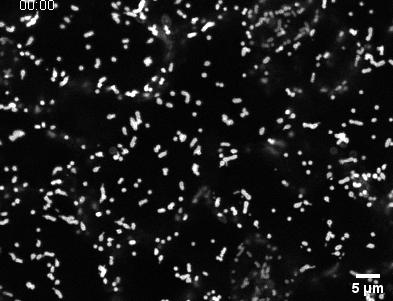
\includegraphics[scale=0.9]{Grafiken/trackpyBilder/video-frame00001.png}
    \caption{raw image with particles to be detected}
    \label{fig:bild_label}
\end{figure}

In diesem Sinne widmet sich die Arbeit in der Folgezeit dem Vergleich möglicher Werkzeugen, die zur Erreichung der eigentlichen Ziele nutzen können. Hierbei werden aus der Vielzahl der Instrumente nur vier bis fünf herausgegriffen. Diese werden zunächst einer tabellarischen Grobanalyse der Merkmale und dann einer textuellen Analyse der Unterschiede unter ihnen unterzogen.\\

\todo{ Completer le tableau}

\begin{tabular}{|c||c|c|c|l|}
 \hline
 Werkzeug & Tutorials & Zugänglichkeit & Parametrisierbarkeit & Dokumentation \\
 \hline
 \hline
 ParticleTracker & +++ & ++ & ++ & +++\\
 \hline
 STracking & ++ & + & + & ++\\
 \hline
 MyPTV  & -- & + & ++ & ++\\
 \hline
 STP  & -- & - & + & --\\
 \hline
 TrackPy  & ++++ & ++ & + & ++++\\
 \hline
\end{tabular}
\\

%\todo{\href{file:///C:/Users/leb/Downloads/10.21105.joss.04398.pdf}{MyPTV}, \\ \href{https://www.sciencedirect.com/science/article/pii/S2001037021002944}{PySTACHIO},\\ \href{https://spt.readthedocs.io/en/latest/}{SPT}
%\\ \href{https://www.google.com/search?q=Python+package+for+particle+tracking&rlz=1C1CHBF_deDE987DE987&sxsrf=ALiCzsYl2NtGnlFYYupES17uNyNLp8zhIQ:1653590912505&ei=gMuPYoKwHsyMxc8Phquk2AM&start=10&sa=N&ved=2ahUKEwiC8MWX6v33AhVMRvEDHYYVCTsQ8NMDegQIARBQ&biw=1920&bih=969}{Python package for particle tracking}}

\section{ParticleTracker \label{kap1_ParticleTracker}}
\textbf{ParticleTracker} ist eine vollständig grafisch bedienbare Software, die es erlaubt, Partikel aus einem Video guter oder niedriger Auflösung zu verfolgen. Diese verwendet mehrere verschiedene Verfolgungsalgorithmen mit einer Standardschnittstelle, um die Einrichtung verschiedener Partikelverfolgungsprojekte schnell und einfach zu gestalten \cite{Smith2021}.
Es werden 3 Methoden des "Tracking" verwendet, nämlich:
\textit{Opencv Hough Circles}: zum Auffinden von Kreisen in einem Bild.
\textit{Trackpy}: Eine bestehende Partikelverfolgungsbibliothek zur Verfolgung von Partikel 
\textit{Opencv Contour finding}: Zum Finden von Konturen in einem Binärbild.
Das erste und das letzte werden von OpenCV \cite{opencv_library} bereitgestellt.

	\paragraph{Vorteile}
		\begin{enumerate}
    			\item \textbf{GUI bedienbar}: \\
				Die Benutzeroberfläche ist eine der beliebtesten Arbeitsmethoden für Benutzer, insbesondere für Neulinge(Siehe \cite{hertzum1996browsing}). Dies ist sicherlich eine hervorragende Möglichkeit, in diesen Bereich einzusteigen, ohne sich mit zu vielen Codezeilen auseinandersetzen zu müssen oder Programmierkenntnisse zu besitzen.
				
    			\item \textbf{Anfängerfreundlich}:\\
				Die Anfängerfreundlichkeit ist stark auf den vorherigen Punkt zurückzuführen, nämlich die GUI-Bedienbarkeit. Zudem ist es sonderlich umstandslos, mit Hilfe einiger Klicks, sich Informationen generieren zulassen, die relevant sind.    
				
    			\item \textbf{Datenvisualisierung}:\\
    			Ein großer Vorteil ist Datenvisualisierung. Dies liegt an der schrittweisen und automatischen Aktualisierung des Renderings in Abhängigkeit von den vorgenommenen Einstellungen. Allerdings ist es notwendig, zunächst das Kästchen "Annotate" zu aktivieren, um die Live-Ansicht zu aktivieren.
    			
    			\item \textbf{Datenausgabe}:\\
 				Der Zugang zu den Daten in der Software ist schnell und einfach. Außerdem sind die Daten in verschiedenen Formen verfügbar. Unter anderem werden die Daten als csv-Datei und auch als Video bereitgestellt, das die Entwicklung der Objekte im Ausgangsvideo nachzeichnet. 
Es ist auch wichtig zu erwähnen, dass es möglich ist, die Daten (in csv) in Bezug auf ein einzelnes Bild zu exportieren.
		\end{enumerate}
		
	\paragraph{Nachteile}
		\begin{enumerate}
				\item \textbf{Das Hochfahren der Software}:\\
				Trotz der Dokumentation war es nicht einfach, die Software zum Laufen zu bringen. In Anbetracht der Verwendung von Bibliotheken, die nur in einer bestimmten Python-Umgebung  verfügbar sind, nämlich "Conda".
Daher wäre es fair zu erwähnen, dass dies für Laien noch schwieriger sein könnte.
				
    			\item \textbf{Funktionsbegrenzt}:\\
				Die Benutzung über eine GUI ist zwar begeisternder Punkt. Doch genau hier liegt die Schwäche. Da die Benutzeroberfläche bereits konfiguriert ist, bietet sie nur die Möglichkeit, die verfügbaren Optionen zu nutzen. Dies könnte in manchen Fällen zu einem Mangel an Optionen führen und somit unzureichend sein.    			
    			
    			\item \textbf{Nicht intuitiv}:\\
    			Obwohl die Verwendung einer grafischen Oberfläche im Allgemeinen für den Benutzer attraktiver ist, sollte sie so intuitiv wie möglich sein oder gut dokumentiert werden (zumindest als Tooltip).
In diesem Fall sind die Namen einiger Optionen auf der Schnittstelle nicht sehr aussagekräftig oder beschreibend(siehe Bild).
\begin{figure}[H]
    \centering
    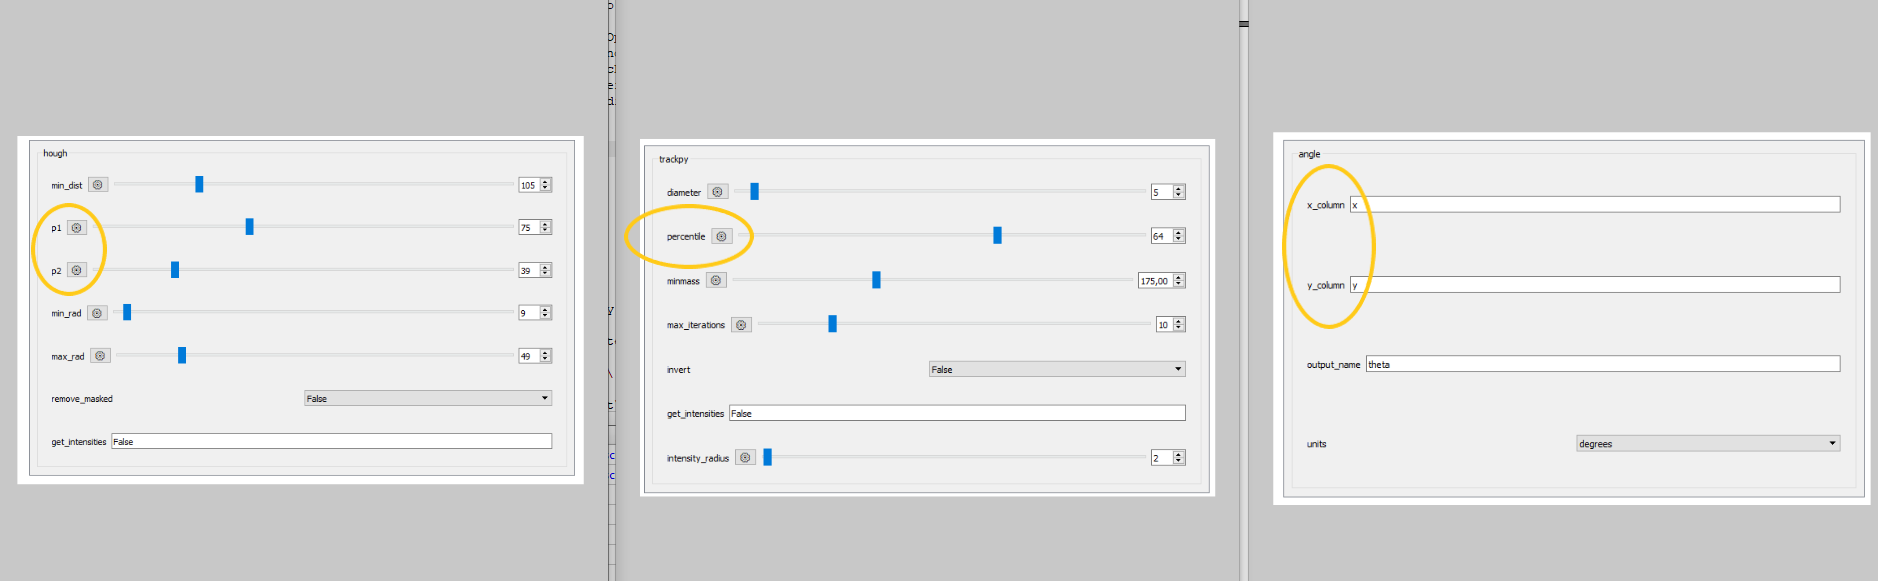
\includegraphics[scale=0.35]{Grafiken/particletracker/Not intuitive.png}
    \caption{Poorly described option names}
    \label{fig:bild_label}
\end{figure}
Es ist daher verständlich, dass man Hinweise erwartet, die die Verwendung der Optionen (Schaltflächen) im Detail beschreiben. 
Dies ist leider nicht der Fall. Daher erfordert die Benutzung der Software ein gewisses Hin und Her in der externen Dokumentation, um die Rolle der Optionen zu kennen.
		\end{enumerate}
		
	\paragraph{Beispiel}
	Wir zeigen hier ein Beispiel für die Erkennung von Partikeln auf einem bestimmten Bild.
	 
	\begin{figure}[H]
    \centering
    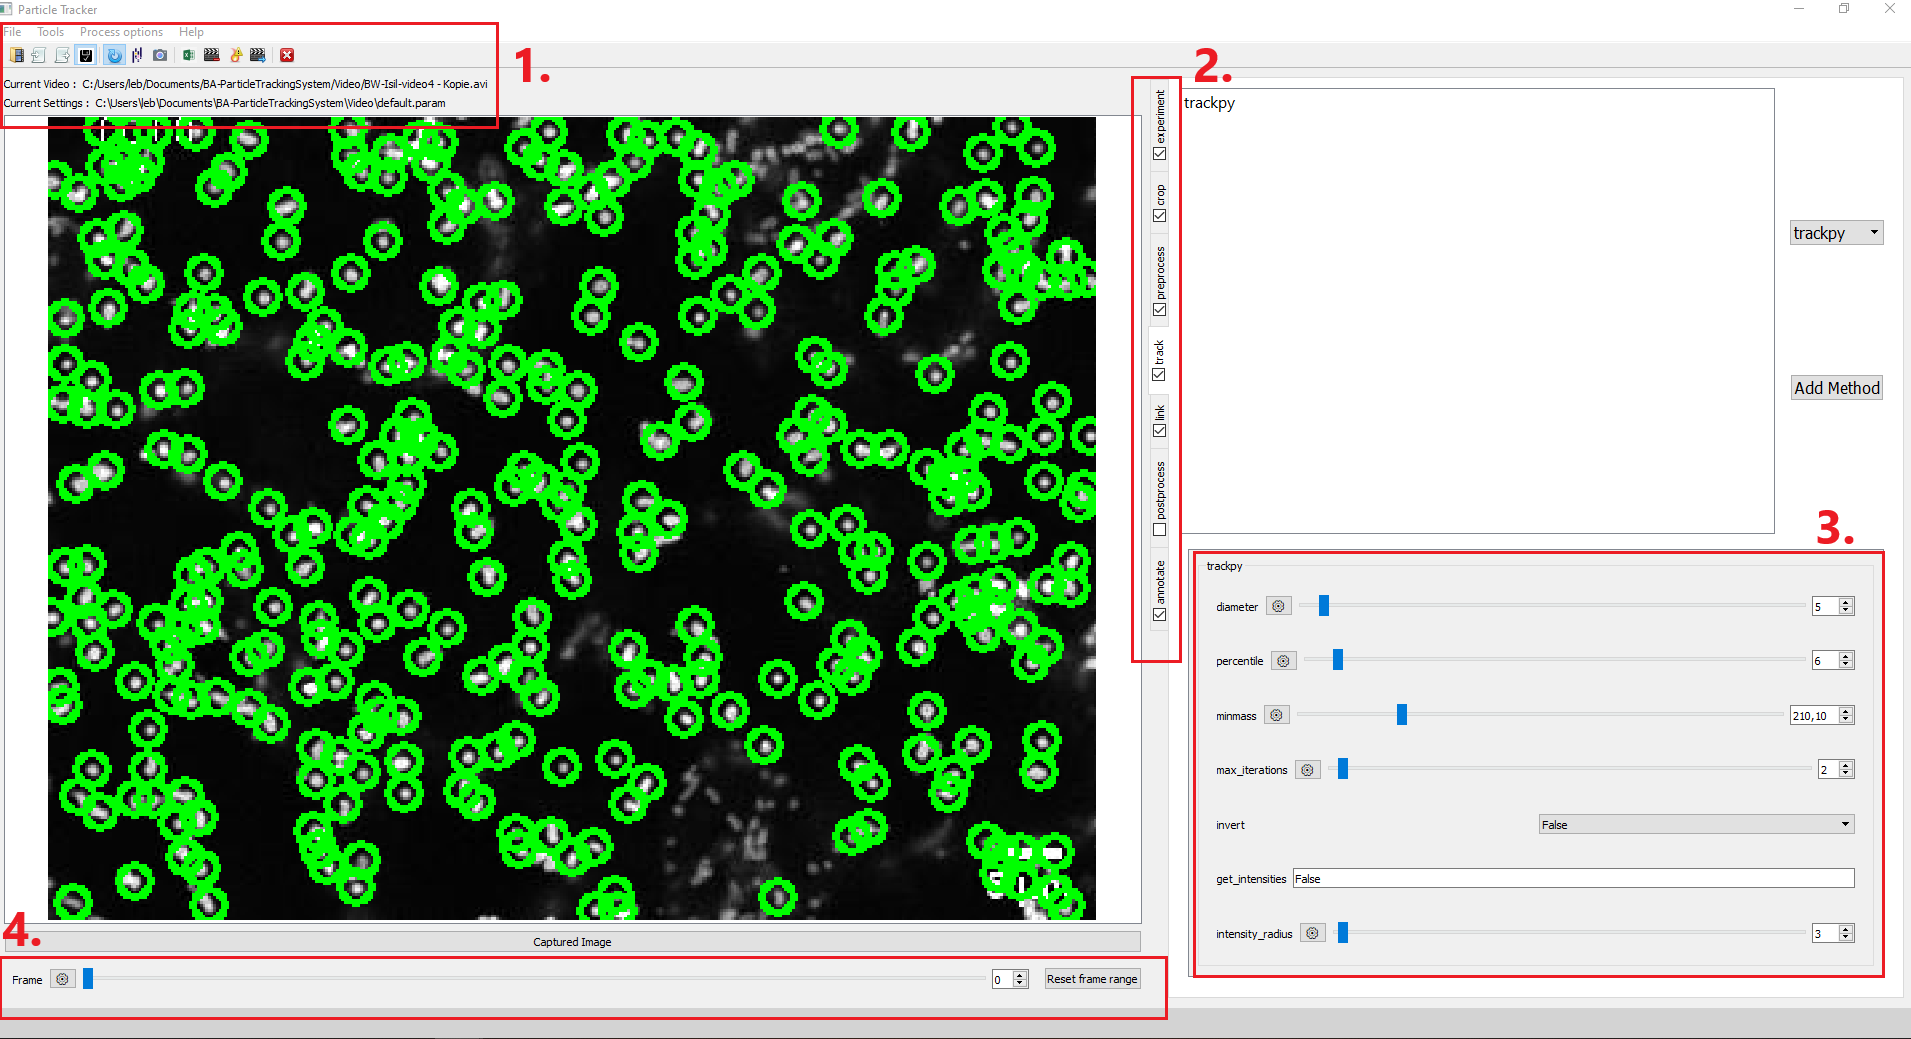
\includegraphics[scale=0.3]{Grafiken/particletracker/Using trackpy.png}
    \caption{Example of particle detection using Trackpy-method of particleTracker}
    \label{fig:bild_label}
\end{figure}

\newpage
	
\section{STracking}
\textbf{STracking} ist ein zu 100\% in Python entwickeltes Framework, dessen Ziel es ist, die Pipeline für die Partikelverfolgung zu entwickeln.
Obwohl es für jede Anwendung zur Verfolgung von Punkten in 2D+t- und 3D+t-Bildern verwendet werden kann, ist seine Hauptidee die Verfolgung intrazellulärer Objekte in Mikroskopiebildern. Sowohl in 2D+t als auch in 3D+t \cite{prigent_2020}.\\
In Kombination mit dem Plugin \textbf{napari}\cite{prigent_2021_napari} bietet es die Möglichkeit, den Tracking-Prozess über eine grafische Benutzeroberfläche zu verwalten.

	\paragraph{Vorteile}
		\begin{enumerate}
    			\item \textbf{Leicht installierbar}:\\
				Mit den in der Dokumentation beschriebenen Schritten ist es relativ einfach, die Bibliothek zu installieren. Die Dokumentation erwähnt Wege, wie die Installation durchgeführt werden könnte, nämlich über \textit{PyPI} und/oder über die \textit{Quelle}. 
Jeder Weg hat natürlich seinen eigenen Anwendungsbereich, der für den jeweiligen Benutzer geeignet ist.

    			\item \textbf{GUI bedienbar}:\\
				Wie erwähnt ist es möglich, das Programm über eine grafische Benutzeroberfläche zu verwenden. Dies geschieht nach der Installation des napari-Plugins.
Hier müssen die ersten Schritte jedoch per Code gemacht werden. 
Das Plugin kann also sowohl zur Manipulation als auch zur Visualisierung der Ergebnisentwicklung verwendet werden. 

		\end{enumerate}
		
	\paragraph{Nachteile}
		\begin{enumerate}
    			\item \textbf{Lückenhafte Dokumentation}:\\
				In der Tat ist die Dokumentationin Bezug auf die Installation der Bibliothek nicht vollstandig. Zum Beispiel wird nirgends erwähnt, dass pyQt installiert werden muss.  Obwohl dieses Modul nur benötigt wird, wenn man die grafische Benutzeroberfläche verwenden will.
				
    			\item \textbf{Unerwartete Reaktion der grafischen Benutzeroberfläche}:\\
				Im Gegensatz zu dem, was in der Dokumentation unter "Example 1: Stracking workflow" beschrieben ist, schließt sich das Fenster, das die visuelle Darstellung der Tracking-Aktionen anzeigen soll, automatisch, sobald es geöffnet wird.  Dies ermöglicht natürlich weder das Betrachten noch das Manipulieren der grafischen Darstellung.Es ist wichtig zu erwähnen, dass pyqt5 in der gleichen virtuellen Umgebung installiert werden muss, um das oben erwähnte Problem zu beheben.
    			
		\end{enumerate}
		

%\newpage	
	
\section{MyPTV}
\textbf{MyPTV} \cite{ron_shnapp_MyPTV} ist eine Software, die vorrangig dazu entwickelt wurde, die 3D-Partikel\-geschwindigkeit aufzuspüren. Es handelt sich um eine Open-Source-Software.
Die Funktionsweise von MyPTV stützt sich stark auf den bewährten mathematischen Rahmen, der im Rahmen des OpenPTV-Projekts(https://www.openptv.net/) entwickelt wurde. Auch die Prinzipien der Photogrammetrie, die in beiden Programmen verwendet werden, sind identisch. Die Software unterscheidet sich jedoch stark durch die Tatsache, dass sie in Python programmiert wurde, das Open Source ist und der wissenschaftlichen Gemeinschaft und nicht-professionellen Computerprogrammierern zugänglich ist.

	\paragraph{Vorteile}
		\begin{enumerate}
    			\item \textbf{Python als Programmiersprache}:\\
    			Die verwendete Programmiersprache ist Python, wodurch die Software für alle, die sie nutzen wollen, leicht zugänglich ist. Sie bietet ein Computer-Ökosystem, das in der Lage ist, den wissenschaftlichen Anforderungen und Herausforderungen gerecht zu werden \cite{5582063_Python_Ecosystem_Scientific_Computing} .
Daher ist es interessant, zu erwähnen, dass ein großer Teil der wissenschaftlichen Gemeinschaft aus den oben genannten Gründen Python verwendet. Dies macht Python zur bevorzugten Sprache für Wissenschaftler und Ingenieure \cite{5725235_Python_Scientists_and_Engineers}. 

    			\item \textbf{Breites Spektrum an Möglichkeiten}:\\
				Die Ressourcen werden so organisiert, dass es für jeden Anwendungsbereich ein spezielles Modul gibt, das alle Funktionen enthält, die in diesem Bereich benötigt werden könnten. So gibt es sechs Module, von der Bildgebung über die Kalibrierung, die Segmentierung, den Partikelvergleich und die 3D-Verfolgung bis hin zum Modul zur Glättung der Pfadlinie.
    			
    			
		\end{enumerate}
		
	\paragraph{Nachteile}
		\begin{enumerate}
    			\item \textbf{Zielgruppe}:\\
				Als Software, die speziell für den wissenschaftlichen und engenieurwissenschaftlichen Gebrauch konzipiert wurde, ist sie aufgrund ihrer Komplexität für Laien nicht geeignet.
				
    			\item \textbf{Schwer bedienbar}:\\
				Trotz der vorhandenen Dokumentation ist die Nutzung der Software recht schwierig. Nicht nur, weil sie, wie im vorherigen Abschnitt beschrieben, auf eine bestimmte Gruppe zugeschnitten ist, sondern auch, weil es an einer Anleitung fehlt, die anhand eines trivialen Beispiels Schritt für Schritt die Verwendung der Software zeigt.
Das macht sie natürlich ziemlich undurchsichtig.
    			
		\end{enumerate}
		

%\newpage

\section{SPT: Single particle tracking analysis \label{kap1_STP}}
\textbf{SPT}\cite{spt_stehr_stein_2020} ist Dies ist ein Python\-Paket, das einen vollständigen Arbeitsablauf für die Analyse der Verfolgung einzelner Partikel bietet. Dabei stützt es sich im Wesentlichen auf andere Pakete wie: \textbf{picasso\_addon}\cite{picasso_addon_schwille-paint_2020} und \textbf{picasso} \cite{picasso_jungmannlab_2019} für die Lokalisierung von Rohfilmen und die Analyse von immobilisierten Partikeln und \textbf{trackpy}\cite{trackpy_allan_daniel_b_2021_4682814} für die Verknüpfung von Lokalisierungen oder die Erstellung von Trajektorien.

	\paragraph{Vorteile}
		\begin{enumerate}
    			\item \textbf{Zielgerichtet}:\\
				Wie in seiner Beschreibung angekündigt, stellt er alle Werkzeuge zur Verfügung, die für die Erreichung dieses Ziels notwendig sind, obwohl er sich auch auf andere Ressourcen stützen kann. Zu Illustrationszwecken verwendet er folgende Tools.
				
				\begin{enumerate}
					\item \textit{picasso}:\\
				 		Für die Lokalisierung und Auswertung von Bildern in verschiedenen Auflösungen.
					\item \textit{picasso\_addon}:\\
						Für alle anderen Funktionen, die neben der Bindung von lokalisierten Partikeln genutzt werden 								können.
					\item \textit{trackpy}:\\
						Für alles, was mit der Verbindung von zuvor lokalisierten Partikeln zu tun hat
				\end{enumerate}
    			
		\end{enumerate}
		
	\paragraph{Nachteile}
		\begin{enumerate}
    			\item \textbf{Schlecht dokumentiert}:\\
				Die Dokumentation des gesamten Handbuchs ist in der Tat sehr unterschiedlich. Sie variiert von sehr wenig Dokumentation für die Installation bis hin zu gar keiner Dokumentation für die Nutzung.  Das macht die Installation und Nutzung natürlich schwierig. Da Sie immer zu den Paketen navigieren müssen, die SPT verwendet (nämlich \textit{picasso}, \textit{picasso\_addon} und \textit{trackpy}), um die notwendigen Informationen für die Installation und gegebenenfalls auch für die Verwendung zu erhalten.
				
    			\item \textbf{Fehlender Benutzerleitfaden}:\\
				Das Fehlen eines Benutzerhandbuchs in einem Paket wie SPT, das sich auf andere Pakete stützt, um Ergebnisse zu liefern, schränkt sowohl die Einarbeitung in die Umgebung als auch deren Beherrschung stark ein. Der Benutzer muss die Funktionen oder Werkzeuge, die er benötigt, selbst aus den Dokumentationen der verschiedenen Pakete lernen und dann zu SPT zurückkehren, um sie anzuwenden.
				
    			
		\end{enumerate}



%\addcontentsline{toc}{section}{Kapitel-1}
%\section{Werkzeugbasierte Erkennung}
\section{Trackpy \label{kap1_trackpy}}
Trackpy ist ein Python-Paket, das es ermöglicht aus einem Video bzw. einer Imagesequenz Partikel in unterschiedlichen Dimensionen (2D und 3D) zu erkennen und zu verfolgen. Hier wird es natürlich die Zweidimensionalität anvisiert. Die Erkennung der Partikel erfolgt über eine der Funktionen des Paketes, nämlich die \textit{locate-}Funktion.
Dieser verfügt über eine reihe von Parametern, anhand derer die Qualität der Anerkennung ausgebessert werden kann.

	\paragraph{Vorteile}
		\begin{enumerate}
    			\item \textbf{Gründlich dokumentiert}:\label{kap1_trackpy_dokumentation}\\
    			Eine ausführliche Dokumentation fast aller Funktionen der Software ist sicherlich ein großer Vorteil der Software. In der Tat trägt sie sehr dazu bei, dass sich der Benutzer schnell eingewöhnt und schnell Vertrauen fasst. Letzteres ist zweifellos eines der Hauptkriterien, auf das die Nutzer achten, wenn es um die Umsetzung geht \textit{siehe}\cite{garousi2013evaluating}.
    			
    			\item \textbf{Benutzerleitfaden}: \label{kap1_trackpy_benutzerleitfaden}\\
				Im Einklang mit einer gründlichen Dokumentation gibt es auf der Website des Pakets eine Reihe von Tutorials (Anleitungen) mit reproduzierbaren praktischen Beispielen, die praktisch alle möglichen Anwendungsbereiche des Pakets abdecken. Auf diese Weise wird der neue und ungeübte Benutzer fast nie allein gelassen. Auf diese Weise wird sowohl ein schneller und allgemeiner Überblick über die Funktionen als auch die sogenannten fortgeschrittenen Funktionen abgedeckt.
				
    			\item \textbf{Breites Spektrum an Möglichkeiten}\label{kap1_trackpy_BSM}:\\
    			Die Lokalisierung von Elementen in einem Bild, die Verfeinerung der Koordinaten von Merkmalen auf eine Genauigkeit von weniger als einem Pixel und die Identifizierung von Merkmalen über die Zeit ebenso wie ihre Verknüpfung zu Trajektorien sind nur die Spitze des Eisbergs. In der Tat bietet "trackpy" weitaus mehr Funktionen, die je nach den Bedürfnissen des Nutzers von großer Bedeutung sein können. Dazu gehören unter anderem Module zur statistischen Datenanalyse, zur Bewegungsanalyse, zu Tracking-Tools und sogar zur Bewegungsvorhersage.
All dies verleiht der Software also ein breites Spektrum an Möglichkeiten.

    			\item \textbf{Hohe Parametrisierbarkeit}\label{kap1_trackpy_HP}\\
    			Die hohe Parametrisierbarkeit beruht hier auf der großen Anzahl an Möglichkeiten, die angeboten werden, um das Ergebnis der Funktionen zu verfeinern. In diesem Sinne bietet die Funktion \textit{locate}\citep{Tp} bis zu 18 nutzbare Parameter, die zur Verfeinerung der Suche und des Ergebnisses verwendet werden können. Obwohl einige von ihnen aus dem einen oder anderen Grund überflüssig oder unwirksam sind.
    			
    			\item \textbf{Beliebtheit in diesem Bereich}\\
    			Aus all den in den vorangegangenen Punkten genannten Gründen und insbesondere dank der \ref{kap1_trackpy_BSM} und \ref{kap1_trackpy_HP} wird sie vielfach bei der Entwicklung anderer Software verwendet, die in ihren Anwendungsbereich fällt. Dies hat dazu geführt, dass wir verschiedene Softwareprodukte finden, die seine Funktionen nutzen, wie z.B. \ref{kap1_STP}, \ref{kap1_ParticleTracker} und viele andere, die im Rahmen dieser Arbeit nicht behandelt wurden.
    			
		\end{enumerate}
		
	\paragraph{Nachteile}
		\begin{enumerate}
				\item \textbf{Fehlerhaftigkeit einiger Beschreibungen}:\\				
				Trotz seiner gut etablierten Dokumentation muss man feststellen, dass es dennoch einige Fälle gibt, in denen die Dokumentation nicht immer korrekt war. Insbesondere hat sich die Anwendung von Prämissen aus der Dokumentation als unpraktikabel erwiesen. Auf diese Fälle wird im weiteren Verlauf dieser Arbeit eingegangen.\todo{Faire une reference au chap parlant de cela}
				    			
    			\item \textbf{Fehlen einer grafischen Benutzeroberfläche}:\\
    			Das Vorhandensein einer gut durchdachten und strukturierten grafischen Benutzeroberfläche, die nicht nur bei der Nutzung der Fülle der angebotenen Funktionen, sondern auch bei der Visualisierung der erzielten Ergebnisse helfen kann, wäre für die Nutzer natürlich noch interessanter und verführerischer gewesen.
		\end{enumerate}
		
	\paragraph{Beispiel:}
	Wir zeigen hier ein Beispiel für die Erkennung von Partikeln auf einem bestimmten Bild.\\
	\begin{figure}[H]
    \centering
    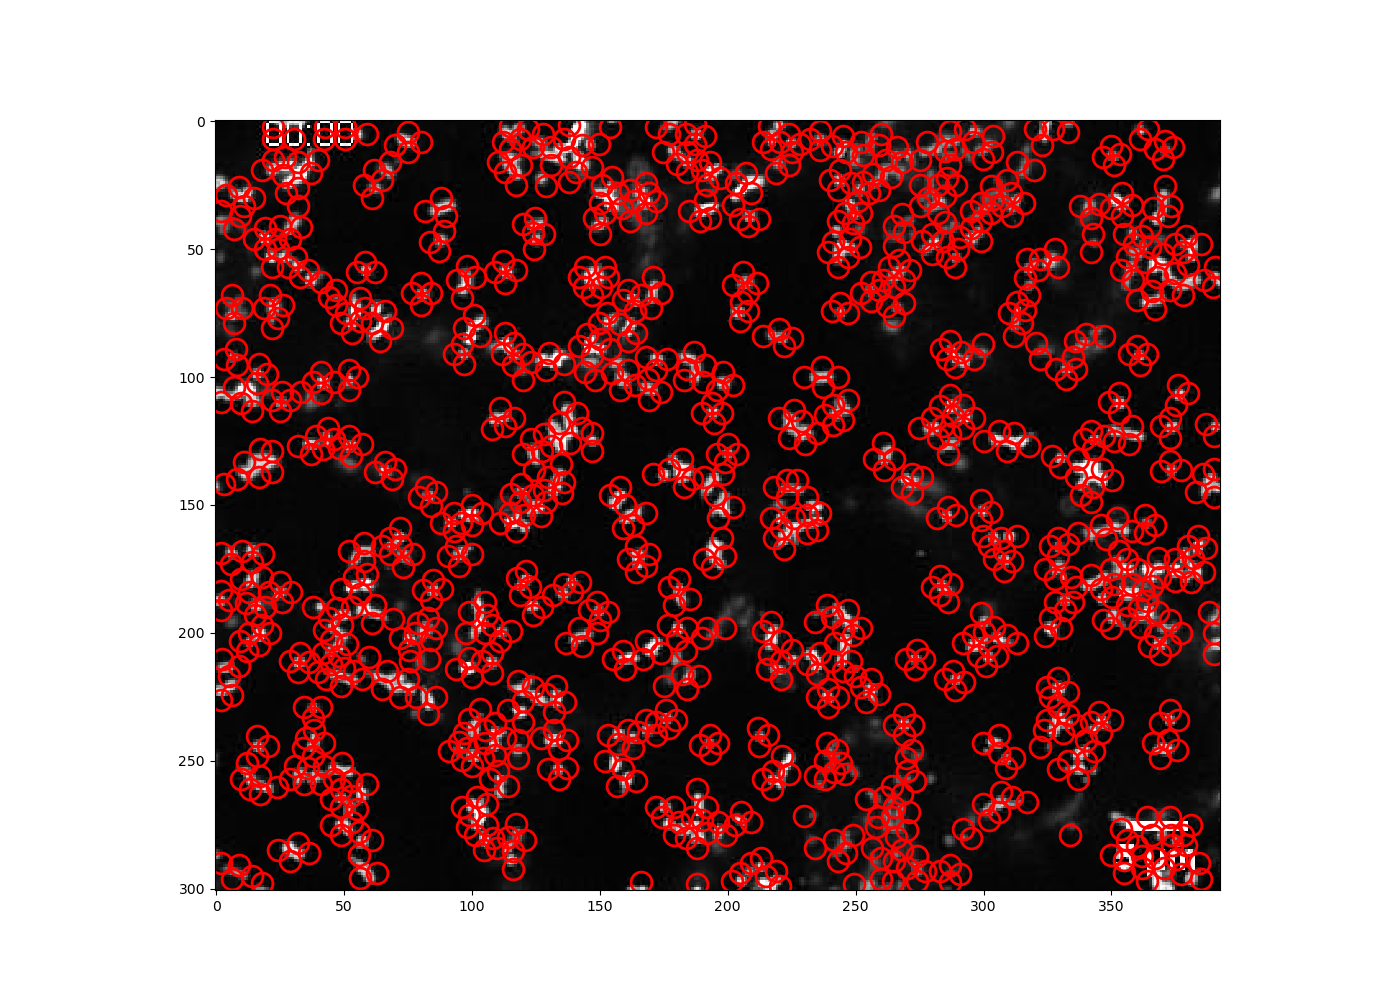
\includegraphics[scale=0.35]{Grafiken/trackpyBilder/locate(f0, diameter=3).png}
    \caption{Example of particle detection using Trackpy}
    \label{fig:bild_label}
\end{figure}
	
In Anbetracht der Gesamtheit der Merkmale, die im Zusammenhang mit der Erwägung von Bibliotheken (Software), die zur Erreichung des oben genannten Ziels beitragen könnten, genannt wurden, ist \textbf{trackpy} der am besten geeignete Kandidat für unsere Arbeit. 

